Dans le parc national des Pyrénées, un chercheur travaille sur le déclin d'une espèce protégée dans les lacs de haute-montagne : le \og crapaud accoucheur \fg.

Les parties \textbf{I} et \textbf{II} peuvent être abordées de façon indépendante.

\begin{center}\textbf{Partie I : Effet de l'introduction d'une nouvelle espèce.}\end{center}

Dans certains lacs des Pyrénées, des truites ont été introduites par l'homme afin de permettre des activités de pêche en montagne. Le chercheur a étudié l'impact de cette introduction sur la population de crapauds accoucheurs d'un lac.

Ses études précédentes l'amènent à modéliser l'évolution de cette population en fonction du temps par la fonction $f$ suivante : \[f(t) = \left(0,04t^2 - 8t + 400\right)\text{e}^{\frac{t}{50}} + 40 \, \text{ pour }\,  t \in [0;120].\]
%
La variable $t$ représente le temps écoulé, en jour, à partir de l'introduction à l'instant $t = 0$ des truites dans le lac, et $f(t)$ modélise le nombre de crapauds à l'instant $t$.

\begin{enumerate}
	\item Déterminer le nombre de crapauds présents dans le lac lors de l'introduction des truites.
	\item On admet que la fonction $f$ est dérivable sur l'intervalle $[0;120]$ et on note $f'$ sa fonction dérivée.
	
	Montrer, en faisant apparaitre les étapes du calcul, que pour tout nombre réel $t$ appartenant à l'intervalle $[0;120]$ on a : \[f'(t) = t(t - 100)\text{e}^{\frac{t}{50}} \times 8 \times 10^{-4}.\]
	\item Étudier les variations de la fonction $f$ sur l'intervalle $[0;120]$, puis dresser le tableau de variations de $f$ sur cet intervalle (on donnera des valeurs approchées au centième).
	\item Selon cette modélisation:
	\begin{enumerate}
		\item Déterminer le nombre de jours $J$ nécessaires afin que le nombre de crapauds atteigne son minimum. Quel est ce nombre minimum ?
		\item Justifier que, après avoir atteint son minimum, le nombre de crapauds dépassera un jour $140$ individus.
		\item À l'aide de la calculatrice, déterminer la durée en jour à partir de laquelle le nombre de crapauds dépassera $140$ individus ?
	\end{enumerate}
\end{enumerate}

\begin{center}\textbf{Partie II : Effet de la Chytridiomycose sur une population de têtards}\end{center}

Une des principales causes du déclin de cette espèce de crapaud en haute montagne est une maladie, la \og Chytridiomycose \fg, provoquée par un champignon.

Le chercheur considère que :

\begin{itemize}
	\item Les trois quarts des lacs de montagne des Pyrénées ne sont pas infectés par le champignon, c'est-à- dire qu'ils ne contiennent aucun têtard (larve du crapaud) contaminé.
	\item Dans les lacs restants, la probabilité qu'un têtard soit contaminé est de $0,74$.
\end{itemize}

Le chercheur choisit au hasard un lac des Pyrénées, et y procède à des prélèvements.

\emph{Pour la suite de l'exercice, les résultats seront arrondis au millième lorsque cela est nécessaire.}

Le chercheur prélève au hasard un têtard du lac choisi afin d'effectuer un test avant de le relâcher.

On notera $T$ l'évènement \og Le têtard est contaminé par la maladie\fg{} et $L$ l'évènement \og Le lac est infecté par le champignon \fg.

On notera $\overline{L}$ l'évènement contraire de $L$ et $\overline{T}$ l'évènement contraire de $T$.

\begin{enumerate}
	\item Recopier et compléter l'arbre de probabilité suivant en utilisant les données de l'énoncé:
	\begin{center}
		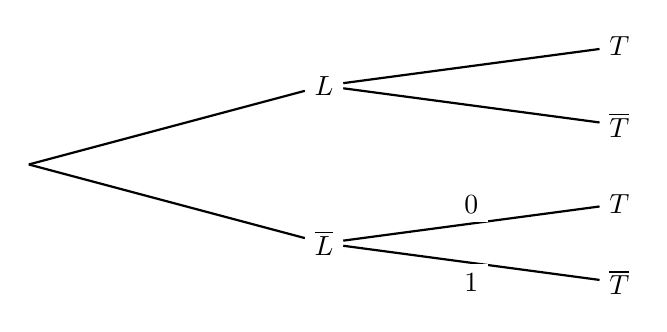
\begin{tikzpicture}
			\tikzstyle{fleche}=[thick]
			\tikzstyle{noeud}=[]
			\tikzstyle{etiquette}=[pos=0.50,fill=white]
			\def\DistanceInterNiveaux{3}\def\DistanceInterFeuilles{1}
			\def\NiveauA{(0)*\DistanceInterNiveaux}\def\NiveauB{(1.25)*\DistanceInterNiveaux}
			\def\NiveauC{(2.5)*\DistanceInterNiveaux}\def\InterFeuilles{(-1)*\DistanceInterFeuilles}
			\coordinate (R) at ({\NiveauA},{(1.5)*\InterFeuilles}) ;
			\node[noeud] (Ra) at ({\NiveauB},{(0.5)*\InterFeuilles}) {$L$};
			\node[noeud] (Raa) at ({\NiveauC},{(0)*\InterFeuilles}) {$T$};
			\node[noeud] (Rab) at ({\NiveauC},{(1)*\InterFeuilles}) {$\overline{T}$};
			\node[noeud] (Rb) at ({\NiveauB},{(2.5)*\InterFeuilles}) {$\overline{L}$};
			\node[noeud] (Rba) at ({\NiveauC},{(2)*\InterFeuilles}) {$T$};
			\node[noeud] (Rbb) at ({\NiveauC},{(3)*\InterFeuilles}) {$\overline{T}$};
			\draw[fleche] (R)--(Ra) ; \draw[fleche] (Ra)--(Raa) ;
			\draw[fleche] (Ra)--(Rab) ; \draw[fleche] (R)--(Rb) ;
			\draw[fleche] (Rb)--(Rba) node[etiquette,above] {$0$}; \draw[fleche] (Rb)--(Rbb) node[etiquette,below] {$1$};
		\end{tikzpicture}
	\end{center}
	\item Montrer que la probabilité $P(T)$ que le têtard prélevé soit contaminé est de $0,185$.
	\item Le têtard n'est pas contaminé. Quelle est la probabilité que le lac soit infecté ?
\end{enumerate}

